\documentclass{scrartcl}
\title{Sprawozdanie 1 \\ Przetwarzanie równoległe}
\subtitle{Mnożenie macierzy porównanie efektywności metod –\\
3 pętle - kolejność pętli: jki,\\
6 pętli - kolejność pętli: zewnętrznych ijk, wewnętrznych: ikj, podział pracy przed pętlą 1.}
\date{2018-05-13}
\author{Bartosz Nawrotek, Krystian Hoczkiewicz \\
Prowadzący: dr inż. Rafał Walkowiak}

\usepackage[utf8]{inputenc}
\usepackage{mathtools}
\usepackage{amssymb}
\usepackage[T1]{fontenc}
\usepackage{listings}
\usepackage{color}
\usepackage{geometry}
 \geometry{
 a4paper,
 total={170mm,257mm},
 left=20mm,
 top=20mm,
 }
\lstdefinestyle{mystyle}{
    backgroundcolor=\color{backcolour},   
    commentstyle=\color{codegreen},
    keywordstyle=\color{codeblue},
    numberstyle=\tiny\color{codegray},
    stringstyle=\color{codepurple},
    basicstyle=\footnotesize,
    breakatwhitespace=false,         
    breaklines=true,                 
    captionpos=b,                    
    keepspaces=true,                 
    numbers=left,                    
    numbersep=5pt,                  
    showspaces=false,                
    showstringspaces=false,
    showtabs=false,                  
    tabsize=2
}

\definecolor{codegreen}{rgb}{0,0.6,0}
\definecolor{codeblue}{rgb}{0,0,0.6}
\definecolor{codegray}{rgb}{0.5,0.5,0.5}
\definecolor{codepurple}{rgb}{0.58,0,0.82}
\definecolor{backcolour}{rgb}{0.95,0.95,0.92}

\usepackage{graphicx}
\graphicspath{ {img/} }

\newcommand\tab[1][1cm]{\hspace*{#1}}
\lstset{style=mystyle}


\begin{document}
\maketitle
\section{Wstęp}
Celem sprawozdania jest analiza wraz z porównaniem efektywności dwóch metod mnożenia macierzy w wersji równoległej oraz sekwencyjnej:
\begin{itemize}
\item {3 pętle w kolejności jki}
\item {6 pętli w kolejności zewnętrznych ijk, wewnętrznych ikj z podziałem pracy przed pierwszą pętlą}
\end{itemize}
Wynikiem mnożenia jest macierz $R$, czynnikami macierze $A, B$. Iloczyn jest liczony wg poniższego wzoru:
\begin{equation}
R_{i, j} = \sum_{k = 1}^{n}{A_{i, k}B_{k, j}}
\end{equation}
gdzie $n$ jest ilością wierszy macierzy kwadratowych $A$ oraz $B$.
Do przeprowadzenia pomiarów korzystano z oprogramowania Code XL oraz do pomiaru czasu działania algorytmu biblioteka time.h.
\section{Analiza algorytmów oraz dyrektyw Open MP}
\subsection{Metoda 3 pętlowa JKI}
\begin{lstlisting}[language=C++, caption={Metoda trzypętlowa}]
void multiply_matrices_JKI()
{
        // mnozenie macierzy 
#pragma omp parallel for 
	for (int j = 0 ; j < COLUMNS ; j++)
      	    for (int k = 0 ; k < COLUMNS ; k++) 
                  for (int i = 0 ; i < ROWS ; i++) 
                        matrix_r[i][j]+= matrix_a[i][k] * matrix_b[k][j] ;              
}
\end{lstlisting}
Jak widać metoda 3 pętlowa charakteryzuje się złożonością $O(n^3)$, gdzie $COLUMNS = ROWS = n$ dla macierzy kwadratowych. W sekwencyjnej metodzie 3 pętlowej wykorzystany został ten sam kod wraz z wyłączoną obsługą dyrektyw OpenMP. W wersji równoległej następuje przydział pracy przed pierwszą pętlą. Powoduje to statyczny podział pracy wg następującego wzoru:
\begin{equation}
j = <id \frac{COLUMNS}{4}, (id + 1)\frac{COLUMNS}{4} - 1>,
j \in \mathbb{Z}
\end{equation}
gdzie $j$ oznacza numer przydzielonej iteracji do procesora o numerze $id \in \{0, 1, 2, 3\}$ dla COLUMNS podzielnego na 4.
\subsection{Metoda 6 pętlowa IJK-IKJ}
\begin{lstlisting}[language=C++, caption={Metoda sześciopętlowa}]
void multiply_matrices_IJK_IKJ()
{
	int r = 10;
	#pragma omp parallel for
	for (int i = 0; i < ROWS; i+=r) {
		for (int j = 0; j < COLUMNS; j+=r) {
			for (int k = 0; k < COLUMNS; k+=r) {
				for (int ii = i; ii < i + r; ii++) {
					for (int kk = k; kk < k + r; kk++) {
						for (int jj = j; jj < j + r; jj++) {
						matrix_r[ii][jj] += matrix_a[ii][kk] * matrix_b[kk][jj];
						}
					}
				}
			}
		}
	}
}
\end{lstlisting}
Metoda 6 pętlowa wykazuje się tą samą złożonością obliczeniową co metoda 3 pętlowa. Wykorzystanie jej ma jednak wpływ na prędkość przetwarzania ze względu na budowę systemu obliczeniowego. Korzysta on z pamięci cache oraz bufora translacji, które aby optymalnie wykorzystać, należy zapewnić odpowiednie warunki przetwarzania, jak lokalność przestrzenna oraz czasowa.
\subsection{Analiza poprawności algorytmów}
Oba algorytmy w wersji sekwencyjnej są poprawne, ze względu na definicję mnożenia macierzy. W wersji równoległej również, ze względu na to, że każdy proces korzysta z innej, rozłącznej części macierzy wynikowej. Nie jest wymagana żadna dodatkowa metoda synchronizacji.
\subsection{Efektywność - synchronizacja}
Jak było nadmienione w punkcie 2.1 oraz 2.2, obie metody cechują się tą samą złożonością obliczeniową. Jednak różnice efektywności mogą być znaczne ze względu na kolejność dostępu do danych z poszczególnych macierzy. Spodziewamy się prawie 4 krotnego przyspieszenia przetwarzania przy użyciu metod w wersji równoległej w stosunku do wersji sekwencyjnej ze względu na niski koszt synchronizacji (przydział pracy statyczny przed pętlą zewnętrzną oraz synchronizacja na końcu działania funkcji).
\subsection{False sharing}
Jest to zjawisko, które może wystąpić tylko w przypadku przetwarzania równoległego. W metodzie równoległej 3 pętlowej zjawisko może wystąpić na krańcach przydzielonych obszarów macierzy $R$. Nie powinno jednak mieć to większego wpływu na czas przetwarzania ze względu na stosunkowo niewielkie fragmenty macierzy, gdzie zjawisko ma możliwość się pojawić.
W metodzie równoległej 6 pętlowej zjawisko również może wystąpić na granicy ostatniego wiersza przydzielonego do danego procesora oraz pierwszego wiersza przydzielonego do kolejnego procesora. W tym wypadku, będzie prawdopodobnie niezauważalne, bo dla całej macierzy występują tylko 4 potencjalne miejsca wystąpienia tego zjawiska niezależnie od wielkości instancji.
\newpage
\subsection{Lokalność dostępu do danych}
Macierze deklarowane są jako tablice dwuwymiarowe, co implikuje przechowywanie ich w pamięci jako pojedyncza linia. Niesie to za sobą możliwość analizy lokalności dostępu do danych.
\begin{figure}[h]
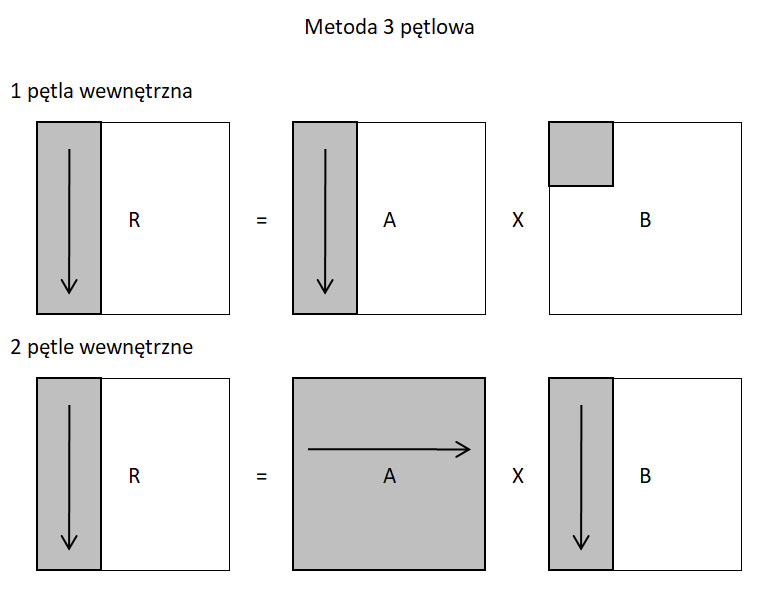
\includegraphics[width=\textwidth]{3petlowa}
\caption{Metoda 3 pętlowa JKI}
\end{figure}
\paragraph{}
Dla metody 3 pętlowej biorąc pod uwagę iteracje wewnętrznej pętli można wyciągnąć następujące wnioski dla poszczególnych macierzy: \\
\begin{itemize}
\item R - brak lokalności przestrzennej ani czasowej
\item A - brak lokalności przestrzennej ani czasowej
\item B - lokalność czasowa
\end{itemize}
Natomiast dla dwóch pętli wewnętrznych:
\begin{itemize}
\item R - brak lokalności przestrzennej ani czasowej
\item A - lokalność przestrzenna, brak lokalności czasowej ze względu na odczyt danych w poszczególnych kolumnach. (kolejne czytane komórki mają oddalone adresy o $n$)
\item B - brak lokalności przestrzennej ani czasowej
\end{itemize}
Braki lokalności spowodowane są iterowaniem po kolejnych elementach w kolumnach poszczególnych macierzy. Powodować to będzie znaczne spadki efektywności działania algorytm.
\paragraph{}
Dla metody 6 pętlowej [1]:
\begin{itemize}
\item lokalność przestrzenna oraz czasowa
\item lokalność przestrzenna
\item lokalność przestrzenna oraz czasowa
\end{itemize}
[2]
\begin{itemize}
\item lokalność przestrzenna oraz czasowa
\item lokalność przestrzenna oraz czasowa
\item lokalność przestrzenna oraz czasowa
\end{itemize}
\end{document}